\chapter{Gravitationnal signature of lunar floor-fractured craters} 
\label{chap7} 
\minitoc

% 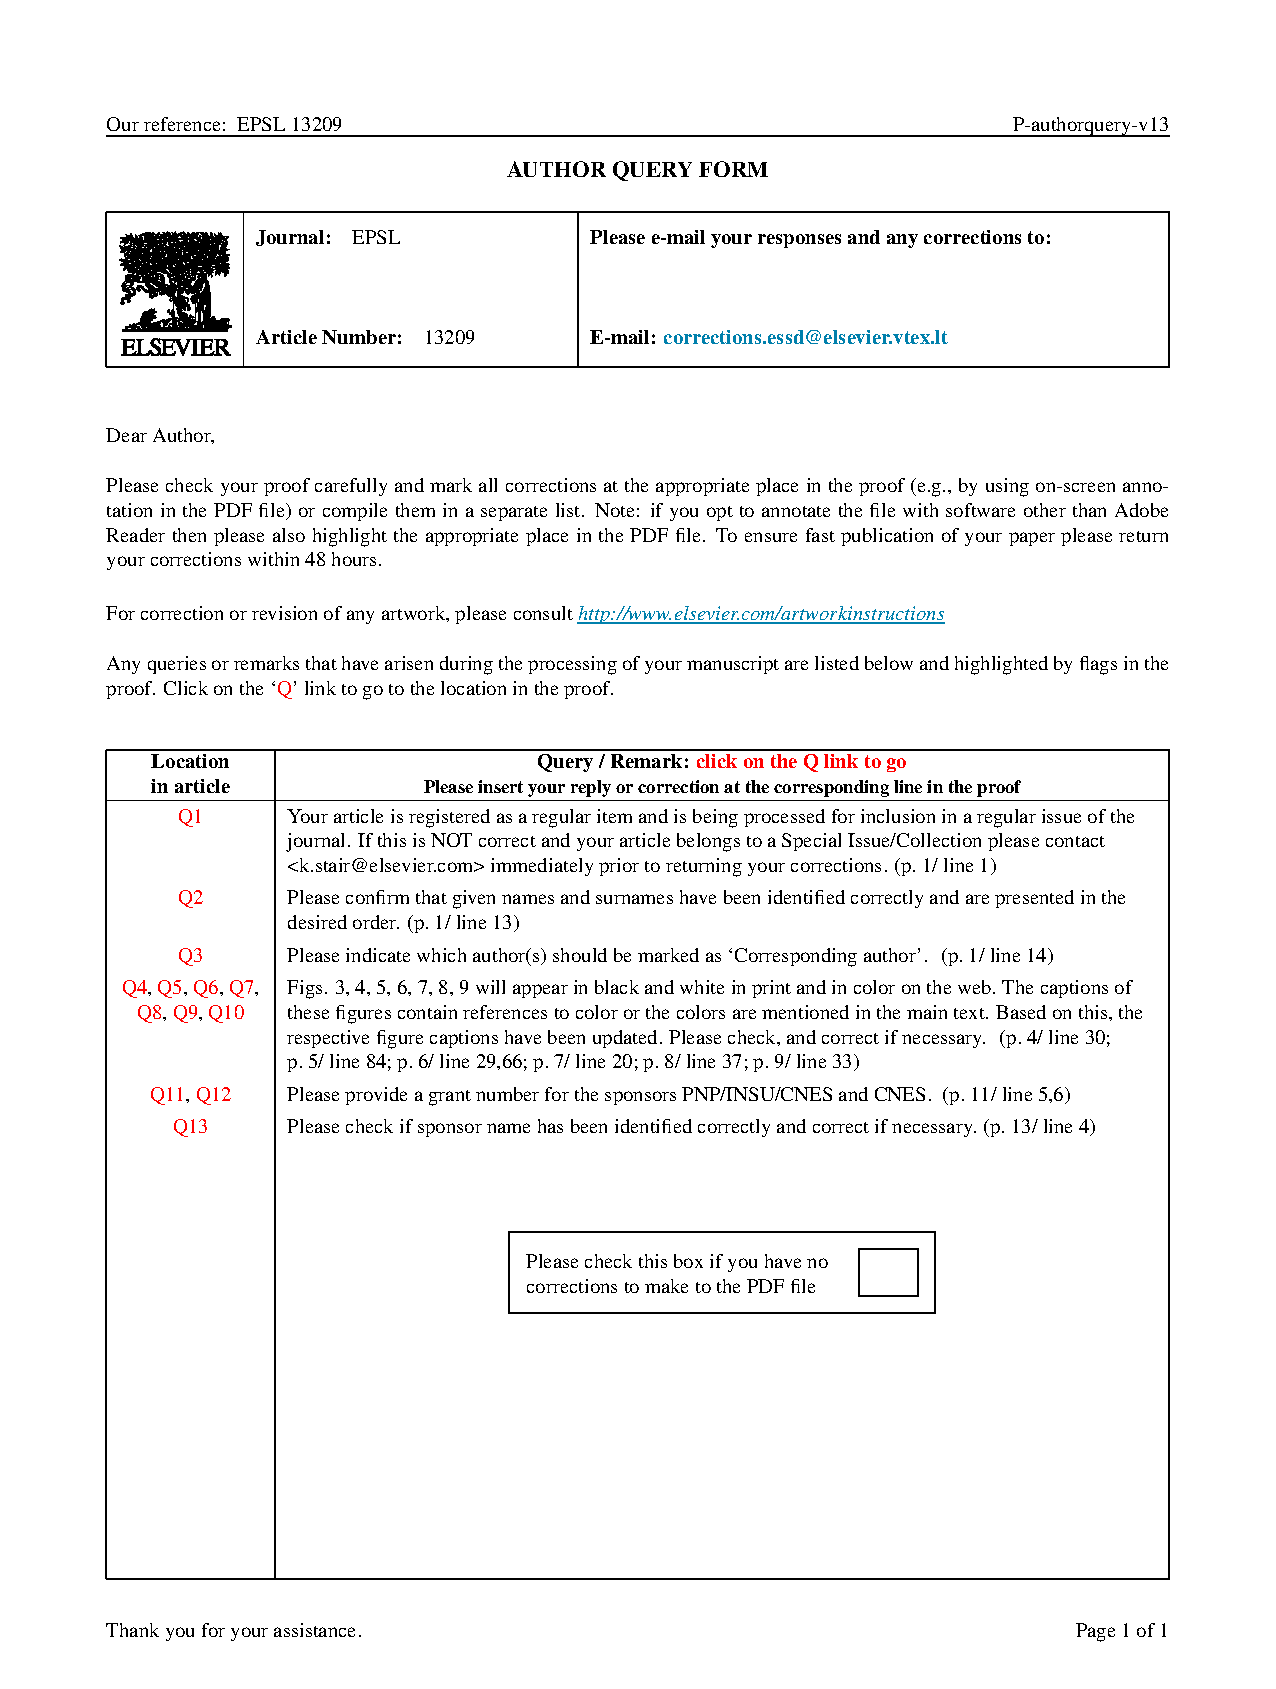
\includepdf[pages=-]{Published_Article/EPSL.pdf}

 \begin{abstract}
    %% Text of abstract

    Lunar floor-fractured craters are  impact craters characterized by
    distinctive  shallow  floors  crossed  by  important  networks  of
    fractures. Different scenarios have been proposed to explain their
    formations but recent  studies showed that the  intrusion of magma
    at depth below the crater floor is the most plausible explanation.
    The intrusion of  dense magma within the light  upper-most part of
    the  lunar crust  should have  left  a positive  signature in  the
    gravity field.   This study  takes advantage of  the unprecedented
    resolution of  the lunar  gravity field  obtained from  the NASA's
    Gravity  Recovery  and  Interior Laboratory  (GRAIL)  mission,  in
    combination with topographic data  obtained from the Lunar Orbiter
    Laser   Altimeter   (LOLA)    instrument,   to   investigate   the
    gravitational  signatures  of   both  normal  and  floor-fractured
    craters.   Despite the  large variability  in their  gravitational
    signatures,  the   floor-fractured  and  normal  craters   in  the
    Highlands   show   significant  differences:   the   gravitational
    anomalies are significantly larger at floor-fractured craters. The
    anomaly amplitudes  for floor-fractured  craters are  in agreement
    with synthetic gravity anomalies  based on the predicted intrusion
    shapes from a theoretical flow  model.  Our results are consistent
    with  magmatic intrusions  intruding  a crust  characterized by  a
    $12\%$ porosity and  where the intrusion has  no porosity. Similar
    studies have  been carried out in  the lunar maria and  South Pole
    Aikten  basin.  Although  the average  gravitational signature  of
    floor-fractured craters is larger than  at normal craters in these
    regions,  they cannot  be distinguished  statistically due  to the
    small  number  of  craters  and   the  large  variability  of  the
    anomalies.  In  general, a  better characterization of  the signal
    due solely to  the initial impact crater is needed  to isolate the
    magmatic intrusion  signal and  characterize the  density contrast
    between the magma and crust.
  \end{abstract}

  \begin{keyword}

    GRAIL\sep Gravity\sep Floor-fractured craters\sep  Intrusive
    magmatism\sep Impact craters\sep Moon

  \end{keyword}

\end{frontmatter}

%% \linenumbers

%% main text

\section{Introduction}
\label{sec:introduction}
  
There are a class of impact craters on the Moon that are distinguished
by  having  uplifted  floors and  radially/concentric  floor-fractured
networks.  About 200 of these floor-fractured craters (FFCs) have been
identified  by \citet{Schultz:1976kt}  and  these  impact craters  are
interpreted  to have  undergone  endogenous  deformations after  their
formation.   The  most striking  feature  of  these craters  is  their
shallow floors compared  to normal craters of the same  size, with the
uplift  reaching $50\%$  of the  initial  crater depth  in some  cases
\citep{Schultz:1976kt}.  Due  to this  deformation, their  floors show
large  networks  of  radial,   concentric  and  pentagonal  fractures.
Additionally,  depending on  local conditions,  the uplift  results in
either a  convex floor or  a flat  plate-like floor, sometimes  with a
wide     circular     moat     just    interior     to     the     rim
\citep{Schultz:1976kt,Jozwiak:2012dq}.

Intrusion of magma beneath the  crater floor and viscous relaxation of
the crater topography  after the impact are two  proposed scenarios to
explain                       these                       deformations
\citep{Schultz:1976kt,Hall:1981kl,Wichman:1995ju,Dombard:2001gs}.  The
recent  theoretical   model  for   the  dynamics   of  crater-centered
intrusions  of  \citet{Thorey:2014cv}  and  recent  morphological  and
geological studies by \citet{Jozwiak:2012dq}  showed that intrusion of
magma  beneath the  crater floor  is  the most  plausible scenario  to
produce  the   morphological  features  observed   at  floor-fractured
craters.
  
Magmatic  intrusions should  be  emplaced at  their  level of  neutral
buoyancy \citep{Walker:1989jq,Taisne:2009kj,Wichman:1995ju}.
Upon  cooling and  solidification,  however, their  densities will  be
larger  than  the surrounding  crustal  material  and hence,  leave  a
positive  signature  in  the  gravity  field.   \citet{Schultz:1976kt}
looked at the gravitational  signature of some floor-fractured craters
with  gravity derived  from radio  tracking data  acquired during  the
Apollo $15$  and $16$  missions \citep{Sjogren:1972kk,Sjogren:1974ij}.
Except at the floor-fractured crater Taruntius, where a strong gravity
anomaly was detected, no pronounced gravity anomalies were observed at
other floor-fractured  crater sites.   However, the gravity  data from
these two  experiments only covered  a narrow swath along  the equator
and the resolution of the data used  in these studies were not able to
detect gravity  anomalies for objects  smaller than about $100$  km in
diameter  \citep{Schultz:1976kt,Sjogren:1974ij}, which  includes about
$88\%$ of the floor-fractured crater population.

Data from  the NASA Gravity  Recovery and Interior  Laboratory (GRAIL)
NASA mission  have provided a global  map of the Moon's  gravity field
with  an  unprecedented resolution.   These  data  have been  used  to
construct a  model of the  gravity field to spherical  harmonic degree
and order  900, which corresponds  to a half-wavelength  resolution of
$\sim 6$ km at the lunar surface \citep{Zuber:2013cp,Konopliv:2014gm}.
These data,  used in  combination with  the topographic  data obtained
from  the Lunar  Orbiter Laser  Altimeter (LOLA)  instrument allow  to
investigate mass anomalies located in the lunar crust.  In particular,
these  data allow  to resolve  small-scale density  variations in  the
shallow crust \citep{Besserer:2014jr,Wieczorek:2013ipa}  and they have
been     used     to     detect     ancient     igneous     intrusions
\citep{AndrewsHanna:2013ft}.

In this paper,  after some theoretical considerations  on the expected
gravitational   signal   at   floor-fractured   craters   in   section
\ref{sec:theor-cons}, we use  GRAIL gravity to detect  the presence of
magmatic  intrusions  at  floor-fractured   crater  sites  in  section
\ref{sec:grav-sign-lunar}.  Then,  we develop  a method to  derive the
density   contrast   between   the   magma  and   crust   in   section
\ref{sec:magm-intr-char}.  We  discuss its geological  implications in
section     \ref{sec:discussion}    and     conclude    in     section
\ref{sec:conclusion}.

\section{Theoretical considerations}
\label{sec:theor-cons}

The Bouguer  anomaly associated  with a  magmatic intrusion  beneath a
crater depends upon the  intrusion characteristics, namely its density
and shape.  Recently, we showed that the morphology of crater-centered
intrusions depends mainly upon the  thickness of the overlying elastic
layer and  on the  crater size  \citep{Thorey:2014cv}.  Guided  by the
results and predictions of our model that is briefly summarized below,
we here  calculate and  discuss the  expected gravitational  signal at
floor-fractured crater sites.

\subsection{Constitutive equations}
\label{sec:const-equat-1}

In  our model,  the intrusion  is  fed at  a constant  rate through  a
cylindrical conduit  located below  the center of  a crater  floor and
spreads   horizontally   along   a    thin   bedding   plane   (Figure
\ref{Figure2-1}).
%% FIGURE 1
\begin{figure}[pb]
    \graphicspath{ {/Users/thorey/Documents/These/Projet/FFC/Gravi_GRAIL/Article/Papier/Proof/} }
  \begin{center}
    \includegraphics[scale=0.60]{Figure_2-1.pdf}
    \caption{Model geometry and parameters.}
    \label{Figure2-1}
  \end{center}
\end{figure}
The  magma makes  rooms for  itself by  lifting the  overlying assumed
elastic  layer, which  is characterized  by a  Young's modulus  $E$, a
Poisson's ratio $\nu$ and an elastic thickness $T_e(r)$ given by
\begin{equation}
  T_e(r)=T_e^0+d_c\xi(r)\hspace{.2cm}\text{, with }\hspace{.2cm} \xi(r)=\frac{1}{1+e^{-\frac{2\alpha(2r-D)}{D}}}-\frac{1}{1+e^{2\alpha}}\label{topo}\\
\end{equation}
where $T_e^0$ is  the overlying layer thickness at  the crater center,
$d_c$  the crater  depth with  respect to  the pre-impact  surface and
$\xi(r)$  a normalized  sigmoid  function which  reproduces a  typical
complex crater depression in terms of the crater diameter $D$ and wall
slope $\alpha$ (Figure \ref{Figure2-1}, top).

The thickness  evolution equation  in cylindrical coordinates  for the
flow of a newtonian fluid is given by \citep{Thorey:2014cv}
\begin{eqnarray}
  \frac{\partial         h}{\partial        t}
  &=&\frac{\rho_{m}g}{12  \mu} \frac{1}{r}  \frac{\partial}{\partial
      r}\left   (r  h^{3}   \frac{\partial  h}{\partial   r}  \right)+
      \frac{\rho_{c}g\Psi       T_{e}^0}{12       \mu}       \frac{1}{r}
      \frac{\partial}{\partial r}\left ( r
      h^{3}  \frac{\partial  \xi(r)}{\partial  r}\right )  \nonumber  \\
  &&+ \frac{E T_{e}^{0^{3}}}{144\mu
     (1-\nu^{2})}\frac{1}{r}\frac{\partial}{\partial  r}\left  (  r
     h^{3}    \frac{\partial}{\partial   r}    \left(\nabla^{2}_{r}
     ((1+\Psi \xi(r))^{3}\nabla^{2}_{r}h )\right)\right )\nonumber\\
  && + w(r,t)
     \label{eq16}\\
  w(r,t)&=&
            \begin{cases} \frac{ \Delta P}{4 \mu Z_{c}} (\frac{a^{2}}{4}-r^{2})&
              r \le \frac{a}{2}\\ 0 & r > \frac{a}{2}
            \end{cases}
                                      \label{eq12}
\end{eqnarray}
where  $h(r,t)$  is  the  intrusion   thickness,  $r$  is  the  radial
coordinate, $t$ is time, $\rho_m$ and $\rho_c$ are the magma and crust
density, $\mu$ is the viscosity,  $\Psi = d_c/T_e^0$ is the thickening
of the overlying layer at the wall, $w(r,t)$ is the injection velocity
and $\Delta P/Z_c$  is the overpressure gradient  driving magma ascent
in the feeder dyke.

The terms  on the right  side of (\ref{eq16})  respectively represent,
from left  to right,  spreading due to  magma weight,  the lithostatic
barrier the  magma has to  face at the  crater wall, squeezing  of the
flow in  response to  elastic deformation of  the overlying  layer and
injection  rate.  Equation  (\ref{eq16}) is  non-dimensionalized using
the crater radius $D/2$ as a  horizontal scale, a height scale $H$ and
a time scale $\tau$ given by
\begin{equation}
  \label{eq18} H= \left (\frac{12\mu Q_{0}}{\rho_{m}g \pi}\right )
  ^{\frac{1}{4}}
\end{equation}
\begin{equation}
  \tau=\frac{\pi     D^{2}      H}{4Q_{0}}\label{eq19}
\end{equation}
where  $H$ is  the characteristic  height scale  of a  gravity current
\citep{Huppert:1982a} and $\tau$ is the characteristic time to fill up
the crater depression for a constant injection rate
\begin{equation} Q_{0}=\frac{\pi \Delta P a^{4}}{128 \mu Z_c} .
  \label{eq11}
\end{equation}
Another useful lengthscale  in the problem is  the flexural wavelength
$\Lambda$ \citep{Michaut:2011kg}
\begin{equation}
  \Lambda &=& \left( \frac{E
      T_{e}^{0^{3}}}{12                        (1-\nu^{2})\rho_{m}g}
  \right )^{\frac{1}{4}}
\end{equation}
which represents the wavelength of deformation of the elastic layer.

Equation (\ref{eq16}) made dimensionless becomes
\begin{eqnarray}    \frac{\partial     h}{\partial    t}&=&\frac{1}{r}
  \frac{\partial}{\partial r}\left  (rh^{3} \frac{\partial h}{\partial
      r} \right)+ \Xi \frac{1}{r} \frac{\partial}{\partial r}\left
                                                            (   rh^{3}\frac{\partial    \xi(r)}{\partial   r}\right   )\nonumber\\
                                                        &+&\Theta
                                                            \frac{1}{r}\frac{\partial}{\partial
                                                            r}\left
                                                            (   rh^{3}
                                                            \frac{\partial}{\partial
                                                            r}
                                                            \nabla^{2}_{r}\left
                                                            ((1+\Psi
                                                            \xi(r))^{3}\nabla^{2}_{r}h
                                                            \right )\right)+
                                                            \frac{32}{\gamma^{2}}
                                                            \left(\frac{1}{4}-\frac{r^{2}}{\gamma^{2}}\right)
                                                            \label{eq21}
\end{eqnarray}
where $\xi(r)$ is also made dimensionless
\begin{equation}
  \xi(r)=\frac{1}{1+e^{-\frac{(r-1)}{\zeta}}}-\frac{1}{1+e^{\frac{1}{\zeta}}}\label{eqqqq}
\end{equation}
and where
\begin{eqnarray}
  \label{Dimensionless1} 
  \gamma&=&\frac{2a}{D}= 0.02\label{n1}\\
  \zeta&=&\frac{d_c}{2\alpha D}=0.13
           \label{n2}\\ \Xi&=&
                               \left(\frac{\rho_{c}gd_{c}}{\rho_{m}gH}\right )
                               = 20 \label{n3}\\
  \Psi&=&\frac{d_{c}}{T_{e}^0} = 1\label{n4}. 
\end{eqnarray}
$\gamma$ is the dimensionless source  width, $\zeta$ is four times the
normalized crater  wall width  and characterizes the  crater geometry,
$\Xi$ is  the ratio between  the lithostatic pressure increase  at the
crater wall  and the  hydrostatic pressure  due to  a magma  column of
thickness  $H$, which  quantifies  the importance  of the  lithostatic
barrier at the crater wall,  and $\Psi$ is the dimensionless thickening
of the upper elastic layer,  which characterizes the elastic thickness
increase at the crater wall.   These are dimensionless parameters that
do not  significantly affect our  results and are considered  fixed in
our analysis \citep{Thorey:2014cv}.  The dimensionless number $\Theta$
\begin{equation}
  \Theta=\left ( \frac{2\Lambda}{D} \right )^{4}\label{n5}
\end{equation}
is the dimensionless  flexural wavelength of the  upper layer raised
to  the power  $4$ that  quantifies the  length scale  over which  the
elastic deformation  is effective  relative to  the crater  radius. It
varies between $10^{-5}$  and $10^{-1}$ and has a  strong influence on
the intrusion shape and final floor appearance.

\subsection{End-member modes of deformation}
\label{sec:end-member-modes-1}

For a constant injection rate and no crater depression, i.e a constant
upper  elastic  layer ($\xi(r)  =  0  $  and  $T_e(r) =  T_e^0$),  the
numerical  resolution of  the  equations shows  two spreading  regimes
\citep{Michaut:2011kg,Michaut:2013dr}.   The flow  is first  driven by
the bending of the upper  elastic layer.  The intrusion is bell-shaped
and both the radius and the  thickness evolve close to $t^{1/3}$. When
the radius becomes larger than $4\Lambda$, the weight of the intrusion
becomes dominant  over the  bending terms and  the intrusion  enters a
gravity current regime.  In this  second regime, the intrusion shows a
flat  top with  bent edges,  the radius  evolve as  $t^{1/2}$ and  the
thickness tends to a constant \citep{Huppert:1982a,Michaut:2011kg}.
 
For a  constant injection  rate and a  crater-like topography  for the
upper  layer,  i.e.  $T_e(r)$  given  by  (\ref{topo}), the  spreading
regimes are perturbed by the presence of the crater wall.  The central
flat floor of the crater first  acts as a constant elastic upper layer
and the intrusion spreads as described above. However, when it reaches
the  crater  wall,  the  important increase  in  lithostatic  pressure
prevents  the  magma  from   spreading  horizontally.   The  intrusion
thickens   in   response   and    the   crater   floor   is   uplifted
\citep{Thorey:2014cv}.   Accordingly, the  intrusion thickness  can be
estimated from the amount of uplift of the crater floor at the center.

%% FIGURE 2
\begin{figure}[pb]
    \graphicspath{ {/Users/thorey/Documents/These/Projet/FFC/Gravi_GRAIL/Article/Papier/Proof/} }
  \begin{center}
    \includegraphics[scale=0.80]{Figure_2-2.pdf}
    \caption{Two  end-member   intrusion  shapes  producing   the  two
      end-member  floor deformations  observed  at  FFC sites:  convex
      floor (left) and plate-like floor (right).}
    \label{Figure2-2}
  \end{center}
\end{figure}

The final morphology  of the crater floor depends mainly  on the ratio
between the  flexural wavelength and  the crater radius, i.e.   on the
dimensionless  number  $\Theta$  (\ref{n5}).   For a  large  value  of
$\Theta$, i.e. a  deep intrusion and/or a small  crater, the intrusion
reaches the wall  in the bending regime. The  intrusion is bell-shaped
and the uplift  of the crater floor leads to  a shallowed convex floor
(Figure \ref{Figure2-2},  left).  In  contrast, for  a small  value of
$\Theta$,  i.e.   a  shallow  intrusion and/or  a  large  crater,  the
intrusion is  in a gravity current  regime when it reaches  the crater
wall.   The  thickening of  the  cylinder-like  intrusion leads  to  a
piston-like uplift of the crater floor and to a shallowed central flat
floor for the crater (Figure \ref{Figure2-2}, right).

Accordingly, this model results into two main types of floor-fractured
craters:  craters  with  convex floors  corresponding  to  bell-shaped
intrusions (Figure \ref{Figure2-2}, left)  and craters with plate-like
floors   corresponding    to   cylinder-shaped    intrusions   (Figure
\ref{Figure2-2},  right).  In  the following,  we consider  craters of
classes   $2$  and   $4$   of   \citet{Schultz:1976kt}  to   represent
manifestations of bell-shaped intrusions,  and craters of classes $1$,
$3$, $5$ and $6$ to be manifestations of cylinder-shaped intrusions.
 
\subsection{Gravitational signature of FFCs: two case studies}
\label{sec:grav-sign-ffcs-1}

The Bouguer gravity  is the gravity anomaly that  remains after taking
into account the gravitational signature of surface topography.  Thus,
if there  are no  lateral variations in  crustal density,  the Bouguer
anomaly of a  floor-fractured crater should be entirely  the result of
the  magmatic  intrusion.   The  Bouguer  anomaly  associated  with  a
magmatic  intrusion   depends  upon  the  intrusion   morphology,  the
intrusion depth  and the  density contrast  $\Delta \rho$  between the
intrusion and the surrounding crust.

We investigate  the signal  expected at  floor-fractured craters  as a
function of the  intrusion shape, diameter and  depth.  In particular,
for the bell and cylinder shaped intrusion, we study the signal for an
intrusion diameter  that varies between  $20$ and $180$ km,  i.e.  the
minimum and  maximum diameter  of floor-fractured craters  observed by
\citet{Schultz:1976kt} and  two intrusion depths, i.e.   $T^0_e =0$ km
and a reasonable upper bound  of $5$ km \citep{Thorey:2014cv}.  We set
the  intrusion thickness  $H_0$ to  a value  of $2$  km, which  is the
maximum  uplift observed  by  \citet{Schultz:1976kt}  and the  density
contrast   between  the   magma  and   the   crust  to   a  value   of
$\Delta \rho = 600$ kg  m$^{-3}$, the maximum density contrast between
mafic  and   crustal  lunar   rocks  using   the  bulk   densities  of
\citet{Kiefer:2012kp}.
 
The two end-member intrusion profiles are obtained by solving equation
(\ref{eq21})  for two  different  values of  the dimensionless  number
$\Theta$ (\ref{n5}),  $\Theta= 10^{-2}$ for the  bell-shaped intrusion
and    $\Theta=    10^{-5}$    for   the    cylinder-like    intrusion
\citep{Thorey:2014cv} .   We stop the  simulations when the  uplift at
the center $h_0$ is significant and  such that the pressure due to the
intrusion weight at the center  is about half the lithostatic pressure
due  to  the  crater  wall   ($h_0=10$).   Finally,  each  profile  is
redimensionalized: the axial coordinate of the dimensionless thickness
profile is multiplied by $D/2$ and the dimensionless thickness profile
is multiplied by $H_0/h_0$, where $h_0$ is the dimensionless thickness
of the intrusion at the end of the simulation.

We calculate the synthetic radial gravity anomaly (more precisely, the
gravity  disturbance)  $\delta_g^s$  corresponding to  each  intrusion
profile using the spherical harmonics expansion
\begin{equation}
  \delta_g^s(r,\theta,\phi)&=&\frac{G
    M}{r^2}\sum_{l=0}^{L_{\text{max}}}\sum_{m=-l}^{l}\left(\frac{R_{i}}{r}\right)^l(l+1)C_{lm}Y_{lm}(\theta,\phi)
\end{equation}
where $r,\theta$ and $\phi$ are the coordinates of observation, $G$ is
the  gravitational constant,  $M$  the  mass of  the  Moon, $R_i$  the
reference radius of  the spherical harmonic coefficients  taken as the
mean     radius     at     the     site     of     intrusion,     i.e.
$R_i =  R_0-T_e^0+\overline{h}$ where $R_0$  is the mean  lunar radius
and  $\overline{h}$  the  mean   intrusion  thickness,  $C_{lm}$,  and
$Y_{lm}$ the spherical harmonic functions  of degree $l$ and order $m$
\citep{wieczorek:1998th}.  Gravitational  accelerations are considered
positive when  directed downward (see Supplementary  materials for the
expression of the spherical  harmonic coefficients associated with the
intrusion thickness profile and the calculation details).

%% FIGURE 3
\begin{figure}[h!]
  \begin{center}
    \graphicspath{ {/Users/thorey/Documents/These/Projet/FFC/Gravi_GRAIL/Article/Papier/Proof/} }
    \includegraphics[scale=0.4]{Figure_2-3.eps}
    \caption{Top  left: Calculated  synthetic  gravity  anomaly for  a
      bell-shaped  intrusion  at  the  surface for  $T_e^0  =  0$  km,
      $H_0 = 2$ km, $D = 180$  km and $\Delta \rho = 600$ kg m$^{-3}$.
      Dotted  red line  represents the  crater rim.   Top right:  Mean
      synthetic gravity anomaly  as a function of  the crater diameter
      $D$  for  a  bell-shaped  intrusion   with  $H_0  =  2$  km  and
      $\Delta \rho = 600$ kg  m$^{-3}$.  Red solid line: the intrusion
      is  at  the  surface,  $T_e^0  =0$ km.   Blue  solid  line:  the
      intrusion is $5$ km below the  surface, $T_e^0 = 5$ km.  Bottom:
      Same as above, but for a cylinder-shaped intrusion.}
    \label{Figure2-3}
  \end{center}
\end{figure}

The two  different intrusion shapes  result in two different  types of
anomaly (Figure \ref{Figure2-3}, left).   For a bell-shaped intrusion,
with a convex  crater floor, the gravity anomaly  is also bell-shaped.
It  decreases gradually  from the  center to  the crater  wall (Figure
\ref{Figure2-3}, top left).   For an intrusion placed  at the surface,
$T_e^0 =0$,  the signal  barely depends on  the crater  diameter.  The
mean gravity  anomaly measured interior  to the crater wall  is almost
constant  and about  $15$  mGal (Figure  \ref{Figure2-3}, top  right).
Although an increased intrusion depth  decreases the mean value of the
anomaly by  a factor that  is less than  two for craters  smaller than
$50$ km, it barely affects the anomaly for craters larger than $50$ km
(Figure \ref{Figure2-3}; top right).

For  a cylinder-like  intrusion  and a  plate-like  crater floor,  the
gravity anomaly  is relatively  uniform and  sharply decreases  at the
crater  wall  (Figure  \ref{Figure2-3}, bottom  left).   Consequently,
although the  maximum amplitude of the  anomaly is similar to  the one
produced  by  a  bell-shaped  intrusion,  the  mean  gravity  anomaly,
measured interior to  the crater wall, is twice larger  and about $30$
mGal. Similar  to bell-shaped intrusion, an  increased intrusion depth
decreases the mean value of the anomaly  by a factor that is less than
two for  craters smaller than $50$  km but barely affects  the anomaly
for  craters  larger  than  $50$ km  (Figure  \ref{Figure2-3},  bottom
right).
  
One important observation of our modeling  is that even for an extreme
case of a $2$ km thick and a $180$ km diameter intrusion placed at the
surface  with a  large  density  contrast of  $600$  kg m$^{-3}$,  the
expected signal is only of a few tens of mGal. Though GRAIL can easily
detect such small  amplitude anomalies, this gravity  signals could be
masked  by  both  large-scale regional  signals  and  short-wavelength
signals  that  are   unrelated  to  our  idealized   model  of  Figure
\ref{Figure2-1}.   Therefore,  we  need  to  filter  out  these  other
contributions to be able to  detect the potential presence of magmatic
intrusions at  floor-fractured craters.  In the  following, we present
the  gravity model  that we  use and  consider the  remaining expected
signal  after  filtering the  synthetics  the  same way  the  observed
gravity are filtered.

\subsection{Filtered GRAIL gravity}
\label{sec:grails-gravity-model-1}

The  observed  gravity field  on  the  Moon  is  a result  of  several
contributions,   including  surface   topography,  relief   along  the
crust-mantle interface and density  heterogeneities in both the mantle
and the crust. In order to  detect the presence of magmatic intrusions
in the  shallow crust, which  have predicted  anomalies of only  a few
tens of mGal,  we first remove all known signatures  from the observed
gravity field in order to highlight those signals that remain.

To construct this model, we  start with JGGRAIL 900C11A gravity field,
which is developed to spherical harmonic degree 900 and which is based
on all  data obtained  during the GRAIL  primary and  extended mission
\citep{Konopliv:2014gm}.  From  the free-air  gravity model,  we first
compute the Bouguer anomaly by removing the gravitational contribution
of surface  topography and  the long-wavelength variations  in crustal
density that are  predicted from remote sensing data,  as described in
\citet{Wieczorek:2013ipa}. The most prominent  signals that remain are
either associated with large impact  basins or are anticorrelated with
long-wavelength topography.  We interpret  the majority of this signal
as  being the  result of  crustal  thickness variations,  and use  the
Bouguer anomaly to invert for the gravitational signal of relief along
the crust-mantle interface, as described in \citet{Wieczorek:2013ipa}.

\begin{figure}[h!]
    \graphicspath{ {/Users/thorey/Documents/These/Projet/FFC/Gravi_GRAIL/Article/Papier/Proof/} }
  \begin{center}
    \includegraphics[scale=1]{Figure_2-4.pdf}
    \caption{Power spectra  for various  gravity models.   Black solid
      line:  free-air gravity  from  the GRAIL  gravity model  JGGRAIL
      900C11A.   Red solid  line: Bouguer  gravity anomaly  assuming a
      constant  crustal density  of  $2550$ kg  m$^{-3}$.  Blue  solid
      line:  Crustal  gravity  anomaly  of our  model  CrustAnom  with
      $\lambda=80$  and which  removes  long-wavelength variations  in
      crustal density as predicted by remote sensing data.}
    \label{Figure2-4}
  \end{center}
\end{figure}

Since  the shortest  wavelength  signals in  the  Bouguer anomaly  are
unlikely to be  the result of crustal thickness  variations, and since
short-wavelength  signals become  highly  amplified when  extrapolated
with  depth  below  the  surface,  we apply  the  low-pass  filter  of
\citet{wieczorek:1998th} to  the Bouguer anomaly before  inverting for
crustal thickness variations.  This  filter is parameterized by having
a value of $0.5$ at spherical harmonic degree $\lambda$. The choice of
$\lambda$  is  subjective,  and  $\lambda$ is  chosen  such  that  the
obtained crustal thickness map does not contain excessive power at the
shortest  wavelengths.   In \citet{Wieczorek:2013ipa},  $\lambda$  was
chosen to  have a  value of  $80$.  Here, we  test several  values for
$\lambda$ and find that $\lambda=80$  is also a good trade-off between
the removal of  regional trends and the removal of  signals due to the
magmatic intrusion itself  (see Supplementary Figure 1  for details on
the effects of $\lambda$).

\begin{figure}[h!]
    \graphicspath{ {/Users/thorey/Documents/These/Projet/FFC/Gravi_GRAIL/Article/Papier/Proof/} }
  \begin{center}
    \includegraphics[scale=0.4]{Figure_2-5.eps}
    \caption{Top left:  Calculated synthetic gravity  anomaly filtered
      the same way as the  model CrustAnom for a bell-shaped intrusion
      at the surface with  $T_e^0 = 0$ km, $H_0 = 2$ km,  $D = 180$ km
      and $\Delta \rho = 600$ kg m$^{-3}$.  Dotted red line represents
      the  crater  rim. Top  right:  Mean  filtered synthetic  gravity
      anomaly  as  a  function  of  the  crater  diameter  $D$  for  a
      bell-shaped intrusion with $H_0 = 2$  km and $\Delta \rho = 600$
      kg m$^{-3}$.  Red  solid line: $T_e^0 =0$ km.   Blue solid line:
      $T_e^0   =  5$   km.   Bottom:   Same  as   above,  but   for  a
      cylinder-shaped intrusion.}
    \label{Figure2-5}
  \end{center}
\end{figure}

After  removing   the  gravitational  signal  of   the  crustal-mantle
interface from  the Bouguer  anomaly, the remainder  of the  signal is
attributed to  lateral variations in  density within the crust  of the
Moon. To remove short wavelength  noise in the gravitational field, we
also  apply a  cosine filter  to the  spherical harmonic  coefficients
between degree $550$ and $650$. It  is from this map, here referred to
as CrustAnom,  that we  search for gravitational  anomalies associated
with  floor-fractured   craters.   Our  model  CrustAnom   is  roughly
equivalent to a  band-passed Bouguer anomaly, where  both the shortest
and longest wavelength signals are removed (Figure \ref{Figure2-4}).

Upon applying the  same filtering to synthetic  gravity anomalies, the
expected signal at floor-fractured craters  is reduced with respect to
those  considered  in   section  (\ref{sec:grav-sign-ffcs-1})  (Figure
\ref{Figure2-5}).  The filtering, which  affects mostly large craters,
leads to a  drop in the amplitude  of the gravity anomaly  by a factor
larger than two for craters larger than about $80$ km.  As an example,
the mean anomaly for  the extreme case of a $2$ km  thick and $180$ km
large intrusion  should only be of  a few mGal in  the model CrustAnom
(Figure \ref{Figure2-5}).


\section{Gravitational signature of lunar craters}
\label{sec:grav-sign-lunar}

The  gravitational  signal  associated  with  magmatic  intrusions  at
floor-fractured craters will be superimposed on the signal of a normal
impact  crater.  We  use the  model  CrustAnom to  first quantify  the
gravity signal at normal impact craters and then compare to the signal
at found floor-fractured craters.
 
\subsection{Normal and floor-fractured crater populations}
\label{sec:unmod-floor-fract}
 
We use the  dataset of \citet{Head:2010fy} as a  reference catalog for
normal  craters  and  the   dataset  of  \citet{Jozwiak:2012dq}  as  a
reference  catalog  for  floor-fractured craters.   We  consider  only
complex craters  and thus use  a minimum  crater diameter of  $20$ km,
which is the  transitional crater diameter between  simple and complex
lunar  craters  \citep{Pike:1974ux,Pike:1980eh}.   We  use  a  maximum
crater diameter  of $180$ km,  because for larger craters,  the mantle
uplift associated with basin formation becomes apparent in the gravity
data \citep{Melosh:2013cz}.  These criteria  result in a population of
$116$  floor-fractured and  $5101$ normal  craters covering  the whole
lunar surface.
	
\begin{figure}[pb]
    \graphicspath{ {/Users/thorey/Documents/These/Projet/FFC/Gravi_GRAIL/Article/Papier/Proof/} }
  \begin{center}

    \includegraphics[scale=0.3]{Figure_3-1.pdf}
    \caption{\textbf{Top  row)} Left:  All  FFCs  (red triangles)  and
      normal craters (light blue circles) in the highlands. Right: All
      FFCs  (red triangles)  and  normal craters  that  have the  same
      spatial    distribution     as    the    FFCs     (light    blue
      circles). \textbf{Middle row)} Same plots but for craters in the
      maria.  \textbf{Bottom row)} Same plots but for craters in South
      Pole Aikten basin (SPA).}
    \label{Figure3-1}
  \end{center}
\end{figure}

The observed  gravity field of an  impact crater will depend  upon the
density of the crust. GRAIL gravity  data show that crustal density is
not constant, and that regional  variations of $\pm$ $250$ kg m$^{-3}$
exist, primarily between the highlands and the South Pole Aitken basin
(SPA). In  addition, surface densities  in the maria  are considerably
higher  than in  the highlands  \citep{Besserer:2014jr}.  To  minimize
potential biases that might arise  from regional variations in crustal
density or geologic evolution, we divide each crater population (normal
and floor-fractured craters) into three sub-populations.  The first is
constituted by craters that lie  within the highlands, outside of both
the maria  and South  Pole-Aitken basin.  We  use the  USGS geological
maps to define the mare borders and the SPA basin is defined using the
best-fit outer ellipse of \citet{GarrickBethell:2009dx}.
In the  highlands, there  are $80$  floor-fractured and  $4054$ normal
craters (Figure \ref{Figure3-1}, top  left).  The second sub-population
is constituted by craters that lie within the maria and outside of SPA basin
of which there  are 22 floor-fractured and 306  normal craters (Figure
\ref{Figure3-1}, middle left).  The  last sub-population is constituted
by craters  within the SPA of  which there are 14  floor-fractured and
603 normal craters (Figure \ref{Figure3-1}, bottom left).
	 
In   each  region   defined   above,  the   spatial  distribution   of
floor-fractured    and   normal    craters   is    different   (Figure
\ref{Figure3-1}, left).  To minimize any  biases that might result from
different regional characteristics, we also consider, for each region,
a second sub-population of normal craters that shares the same spatial
distribution  as the  floor-fractured  craters   (Figure  \ref{Figure3-1},
right).  In this  sub-population, we consider all  normal craters that
are less than $150$ km away from a floor fractured crater.

\subsection{Crater gravitational signatures}
\label{sec:crat-grav-sign}
  
In analyzing the  gravitational signature of lunar  impact craters, we
make  use of  a single  number, the  crater gravity  anomaly, that  is
defined  as the  average  gravitational anomaly  with  respect to  the
regional value.   In calculating this  number, we first  calculate the
average gravitational anomaly from our model CrustAnom within the main
crater rim, i.e.  within a circular region defined by its radius $D/2$
where $D$ is  the crater diameter reported  by \citet{Head:2010fy} and
\citet{Jozwiak:2012dq}.  We then subtract  from this value the average
value of the gravity field in an annulus extending from the crater rim
to a radius of one crater diameter $D$ (Supplementary Figure 2).  Both
gravitational anomalies are calculated at the average elevation of the
crater.

\subsubsection{Highlands}
\label{sec:highlands-1}
  
The magnitude of the gravity anomalies at normal crater sites shows an
important  variability  (Figure  \ref{Figure3-2}).   On  average,  the
anomaly is  positive at  the smallest  craters, slowly  decreases with
increasing diameters, and approaches a  constant negative value near a
diameter  of about  100 km.   For crater  diameters between  $100$ and
$180$ km, the  mean magnitude of the gravity  anomalies is independent
of  the diameter  and close  to $-5$  mGal.  The  mean of  the gravity
anomalies for  the whole  population $\mu_{\delta_g}$ is  negative and
equal to  $-0.71$ mGal.  This  number is  well constrained due  to the
large number of  craters.  In particular, the uncertainty  in the mean
(the standard  error, which is  the standard deviation divided  by the
square root of  the number of observations) is equal  to $ 0.12$ mGal.
The population that shares the spatial distribution of floor-fractured
craters   shows   similar    trends   (Figure   \ref{Figure3-2}).    A
Kolmogorov-Smirnov (KS) test was  conducted to compare this population
to the whole  population of normal craters.  The test  reports a value
of $p$,  which is the  probability that  the two population  are drawn
from the same distribution, larger than $10\%$, which confirms that no
significant   differences   exist    between   the   two   populations
(Supplementary Table 1).
  
%% FIGURE 8
\begin{figure}[pb]
    \graphicspath{ {/Users/thorey/Documents/These/Projet/FFC/Gravi_GRAIL/Article/Papier/Proof/} }
  \begin{center}

    \includegraphics[scale=0.3]{Figure_3-2.eps}
    \caption{Magnitude  of  the   gravity  anomaly  $\delta_g$  versus
      diameter $D$ for  the normal crater population  (blue dots), the
      normal   crater  population   that   shares   the  FFC   spatial
      distribution (light  blue dots)  and the  floor-fractured crater
      population (red triangles) in the highlands. Solid line: Mean of
      the  gravity anomalies  binned  in $15$  km diameter  intervals.
      Error bars correspond to the standard error for each bin.  Right
      plot:  Corresponding gravity  anomaly  density distribution  for
      each population in frequency ($\%$).}
    \label{Figure3-2}
  \end{center}
\end{figure}

The  magnitude of  the  gravity anomalies  at floor-fractured  craters
shows  a different  dependence with  diameter than  at normal  craters
(Figure  \ref{Figure3-2}).  Although  the  variance of  the data  with
respect to the average is of  the same order, the gravity anomalies at
floor-fractured craters  are larger.  In  particular, the mean  of the
floor-fractured crater gravity anomalies is positive and approximately
$2.7$  mGal  larger  than  the  mean  of  the  normal  crater  gravity
anomalies.  We made use of a t-test to determine the robustness of the
difference between the mean magnitude  of the gravity anomalies of the
two  populations.    This  test  quantifies  the   significance  of  a
difference  between the  means  of two  populations  assuming the  two
populations have the same variance.  We found that there was only less
than  a $5\%$  chance  that the  difference  in the  mean  of the  two
populations  could have  occurred by  chance (Supplementary  Table 1).
The  same result  holds  for  the comparison  with  the normal  crater
population  that shares  the spatial  distribution of  floor-fractured
craters (Supplementary Table 1).

\subsubsection{Lunar maria and SPA}
\label{sec:lunar-maria-spa}
  
The magnitude of the gravity anomalies at the sites of complex craters
in the lunar  maria shows a variability that is  similar to craters in
the  highlands (Figure  \ref{Figure3-3},  top).   The gravity  anomaly
remains close  to $0$ mGal and  is independent of the  crater diameter
(Figure  \ref{Figure3-3},  top).  The  mean  of  the whole  population
$\mu_{\delta_g}$ is positive and equal to  $1.51 \pm 0.68$ mGal.  A KS
test shows that there is  no significant difference between the entire
normal  crater  population  and  the   one  that  shares  the  spatial
distribution of floor-fractured  craters (Figure \ref{Figure3-3}, top,
Supplementary Table 1).
%% FIGURE 9
\begin{figure}[pb]
    \graphicspath{ {/Users/thorey/Documents/These/Projet/FFC/Gravi_GRAIL/Article/Papier/Proof/} }
  \begin{center}

    \includegraphics[scale=0.3]{Figure_3-3.eps}
    \caption{\textbf{Top}: Magnitude of the gravity anomaly $\delta_g$
      versus  diameter  $D$ for  the  normal  crater population  (blue
      dots), the normal crater population  that shares the FFC spatial
      distribution (light  blue dots)  and the  floor-fractured crater
      population (red triangles) in the maria. Solid line: Mean of the
      gravity anomalies  binned in $15$ km  diameter intervals.  Error
      bars correspond to the standard error for each bin.  Right plot:
      Corresponding  gravity  anomaly  density distribution  for  each
      population in frequency ($\%$).  \textbf{Bottom}: Same plots but
      in South Pole-Aikten basin.}
    \label{Figure3-3}
  \end{center}
\end{figure}

The  normal  craters in  the  South  Pole  Aikten basin  show  gravity
anomalies  that  are somewhat  more  negative  than in  the  highlands
(Figure \ref{Figure3-3},  bottom).  On  average, the  signal decreases
with  increasing   diameter  up  to   $D  \sim  100-120$   km  (Figure
\ref{Figure3-3},  bottom)  and  increases somewhat  again  for  crater
diameters between $120$ and $180$ km (Figure \ref{Figure3-3}, bottom).
A KS  test shows that there  is no significant difference  between the
two  populations of  normal craters  (Figure \ref{Figure3-3},  bottom,
Supplementary Table 1).

Although the mean  magnitude of the gravity anomalies at  FFC sites is
about $3$ mGal  larger than the mean value observed  at normal craters
in the maria and SPA, the variability in the signal is large and there
is  no significant  statistical  difference between  the  mean of  the
gravity anomalies of  normal and floor-fractured craters  in those two
different regions.  Indeed, a t-test, realized for both regions, shows
that there was more than a $10\%$ chance that these differences in the
mean  of   the  two   populations  could   have  occurred   by  chance
(Supplementary Table  1).  Nevertheless, the  small number of  FFCs in
the  maria and  in the  SPA makes  difficult to  obtain a  significant
statistic due to the low accuracy in measuring the FFC population mean
($\mu_{\delta_g}   =4.43  \pm   3.52   $  mGal   in   the  maria   and
$\mu_{\delta_g} =-0.25\pm 2.52 $ mGal in SPA).

\section{Magmatic intrusion characteristics}
\label{sec:magm-intr-char}
  
Our  results  show that,  on  average,  crustal gravity  anomalies  at
floor-fractured craters  are larger than  at normal craters,  but also
that   this  result   is  statistically   significant  only   for  the
highlands. This  is in agreement  with the presence of  dense magmatic
intrusions at depth below floor-fractured crater floors.  In addition,
the  amplitudes of  the  gravitational  signatures at  floor-fractured
craters are only of a few mGal, comparable to the predictions based on
the    theoretical    model     of    \citet{Thorey:2014cv}    (Figure
\ref{Figure2-5}).  In  the following, we compare  the observed gravity
signals at each floor-fractured crater  to a synthetic gravity anomaly
constructed based on the theoretical model of \citet{Thorey:2014cv} in
order to  derive the mean  density contrast between the  intrusion and
the  surrounding  crust.   To  that purpose,  the  thickness  of  each
intrusion is needed and we use  LOLA topographic data to estimate this
quantity for each floor-fractured crater.

\subsection{Intrusion thickness}
\label{sec:intrusion-thickness}

The intrusion thickness $H_0$ at the  center of the crater is taken as
the  amount of  shallowing of  the crater  floor with  respect to  the
expected   depth  \citep{Schultz:1976kt,Jozwiak:2012dq}.    Given  the
observed crater depth, the problem  is to estimate the original crater
depth   before    the   intrusion    formed.    In   the    study   of
\citet{Jozwiak:2012dq}, the scaling law which gives the depth $d_c$ as
a function of the crater diameter $D$, derived by \citet{Pike:1974ux},
was used as  an estimate for the initial crater  depth.  However, this
scaling law was calculated using only recent, Erastosthenian, and well
preserved   craters,   and   it   is   generally   acknowledged   that
floor-fractured  craters are  generally older  and more  degraded than
this  population.  In  the  absence  of information  on  the state  of
degradation of lunar craters in the dataset of \citet{Head:2010fy}, we
thus  use the  characteristics of  the normal  craters that  share the
spatial distribution  of floor-fractured craters described  in section
\ref{sec:unmod-floor-fract} as a reference.

\begin{figure}[pb]
    \graphicspath{ {/Users/thorey/Documents/These/Projet/FFC/Gravi_GRAIL/Article/Papier/Proof/} }
  \begin{center}

    \includegraphics[scale=0.4]{Figure_4-1.pdf}

    \caption{Crater  depth $d_c$  (km)  versus diameter  $D$ (km)  for
      floor-fractured craters  (red) and normal craters  (blue) in the
      highlands,  SPA  and  the  maria.  The  normal  craters  in  the
      highlands reference to the  populations close to floor-fractured
      craters.  Error bars are the uncertainties in the measurement of
      the  crater depth  and for  clarity, the  uncertainties are  not
      shown  for normal  craters.  Dashed  lines: best  fit using  the
      equation $d_c =  AD^B$ for the floor-fractured  crater (red) and
      the normal  crater (blue) populations in  log-log space.  Values
      of the  coefficient A, B  as well  as the dispersion  around the
      best fit  line $\sigma_{fit}$  are given in  Supplementary Table
      2.}
    \label{Figure4-1}
  \end{center}
\end{figure}


We characterize the depths of  both normal and floor-fractured craters
using  the 64  ppd ($\sim450$  m/pixel) LOLA  gridded topography  data
\citep{Zuber:2009bq}   obtained  from   the   planetary  data   system
geosciences   node.     We   followed   the   method    described   by
\citet{Kalynn:2013fg}  to  derive  the  crater  depth  $d_c$  and  its
uncertainty  $\sigma_{d}$ (see  Supplementary Materials  for details).
Our  $d_c$-$D$  results  for  normal  craters  show  trends  that  are
consistent with previous  works in the highlands, the  lunar maria and
the SPA (Figure \ref{Figure4-1}).  Indeed,  the crater depth of normal
craters increases  with increasing diameter  and craters in  the maria
are  on  average  shallower  than  in the  highlands  or  SPA  (Figure
\ref{Figure4-1})        \citep{Pike:1974ux,Pike:1980eh,Kalynn:2013fg}.
Nevertheless, the variability in the  degradation state of each crater
results in  an important  variance in the  crater depth  with diameter
with respect to the mean trend.

The same  variability holds for the  floor-fractured crater population
depth   (Figure   \ref{Figure4-1}).    This  variability   makes   the
identification   of   the    uplift   difficult   at   floor-fractured
craters. Although the mean crater  depth of floor-fractured craters in
the highlands and SPA is slightly  smaller than the mean of the normal
crater  population,  the   means  of  the  two   populations  are  not
significantly  different  in  the  three regions  (t-test:  $p>  0.5$,
Supplementary Table  2).  A detailed  geological study at  each crater
would  be necessary  to  precisely identify  the crater  morphological
structures and decrease  the uncertainty in the  depth estimation, but
such a  study is  out of  the scope  of this  article.  We  decided to
estimate the intrusion thickness at  floor-fractured craters only to a
first order by  considering the difference in the  mean trends between
normal and floor-fractured craters.

To characterize  the mean trend  of normal craters,  we make use  of a
linear least-squares regression in log-log space to obtain a power law
relationship of the form $d_c=AD^B$ \citep{Pike:1974ux,Kalynn:2013fg}.
We  use  the  same  method  to characterize  the  mean  dependence  of
floor-fractured  crater depth  with crater  diameter.  In  addition of
determining  the  constant  $A$  and   $B$,  we  also  calculated  the
root-mean-squared dispersion $\sigma_{\text{fit}}$ around the best fit
(Supplementary  Table 2).   Subtracting  the two  best  fit lines,  we
finally obtain a  first-order estimate for the  intrusion thickness at
the center $H_0$ for each floor-fractured crater of given diameter $D$
to          which         we          assign         an          error
$\sigma_{H_0}
=(\sigma_{\text{fit-FFC}}^2+\sigma_{\text{fit-Unmod.Crater}}^2)^{1/2}$.

\subsection{Density contrast $\Delta \rho$ of the intrusion}
\label{sec:intr-dens-contr}

We  consider   two  different   shapes  for  the   intrusions  beneath
floor-fractured craters: a bell-shaped intrusion for craters that show
a   convex  floor   (class  2   and   4  in   the  classification   of
\citet{Schultz:1976kt}) and a cylindrical-shaped intrusion for craters
that  show  a   plate-like  floor  (class  1,  3,  5   and  6  in  the
classification  of  \citet{Schultz:1976kt}).   The  two  dimensionless
profiles  are described  in  section \ref{sec:end-member-modes-1}  and
each profile is redimensionalized using the thickness of the intrusion
$H_0$      and      its       radius      $D/2$      (see      section
\ref{sec:intrusion-thickness}).   The   method  used  to   derive  the
synthetic  gravity anomaly  from  the intrusion  thickness profile  is
detailed is section \ref{sec:grav-sign-ffcs-1}.  We use a unit density
contrast, i.e.   $\Delta \rho  = 1$  kg m$^{-3}$  and then  filter the
predicted gravity  anomaly in exactly  the same way than  the observed
gravity is  filtered (section  \ref{sec:grails-gravity-model-1}).  The
synthetic   gravity   anomaly   $\delta_g^s$  associated   with   each
floor-fractured crater is defined as the mean of the synthetic gravity
anomaly measured interior to the crater rim.
  
Finally, the  density contrast between  the magma  and the crust  at a
specific floor-fractured crater location is given by the difference of
the observed  gravity anomaly  $\delta_g^{obs}$ and  the value  of the
gravity anomaly for normal craters  $\delta_g^c$ of the same diameter,
divided by the  synthetic gravity anomaly for a  unit density contrast
$\delta_g^s$
\begin{equation}
  \Delta \rho = \frac{\delta_{g}^{obs}-\delta_{g}^c}{\delta_{g}^{s}}
\end{equation}
where $\Delta \rho$ is in kg m$^{-3}$.

We   find   that  the   corrected   gravity   anomalies  observed   at
floor-fractured crater  sites in the  highlands are consistent  with a
mean   density  contrast   between  the   magma  and   the  crust   of
$\mu_{\Delta \rho}  = 913 \pm  269 $ kg m$^{-3}$  (Supplementary Table
4).  In  the maria,  the corrected gravity  anomalies observed  in the
$22$  floor-fractured  craters  are  consistent with  a  mean  density
contrast  equal to  $\mu_{\Delta  \rho}  = 484  \pm  669$ kg  m$^{-3}$
(Supplementary  Table 4).   However, the  difference between  the mean
density contrast in the highlands and  the maria is not significant (a
t-test gives a  probability greater than $10\%$ that  this could occur
by chance, $p > 0.1$).  In  the South Pole Aikten basin, the corrected
gravity  anomalies observed  in the  $14$ floor-fractured  craters are
consistent    with    a    mean     density    contrast    equal    to
$\mu_{\Delta \rho}  = 974 \pm  846 $ kg m$^{-3}$  (Supplementary Table
4).   But, the  difference between  the mean  density contrast  in the
highlands  and  SPA  is  also  not  significant  (a  t  test  gives  a
probability  greater than  $50\%$  that this  could  occur by  chance,
$p > 0.5$).

\section{Discussion}
\label{sec:discussion}

In  this study,  we  used  the gravity  field  obtained  by the  GRAIL
mission, in combination with the topographic data obtained by the LOLA
instrument, to  resolve mass anomalies below  floor-fractured craters.
We  studied separately  the craters  in the  farside highlands,  South
Pole-Aikten basin  and maria to  prevent potential bias  from regional
effects.

We show that the average  gravitational signature of normal craters in
the highlands is negative, whereas the average gravitational signature
of floor-fractured craters is  positive.  Although a large variability
characterizes the magnitude of  gravity anomalies in both populations,
the  difference between  the mean  of  the two  populations, equal  to
$\sim  3$  mGal,  is  statistically  significant.   In  addition,  the
floor-fractured  crater  gravity  anomalies  do not  follow  the  same
dependence  with   diameter  as  normal  craters.    Our  results  are
consistent  with   the  emplacement   of  magmatic   intrusions  below
floor-fractured     craters     as      originally     proposed     by
\citet{Schultz:1976kt}.  Furthermore,  the observed  gravity anomalies
(after  filtering) of  a few  mGal are  in agreement  with the  values
expected   from   the   model    of   crater-centered   intrusion   of
\citet{Thorey:2014cv}.  In  particular, measured gravity  anomalies at
floor-fractured craters imply an  average density contrast between the
magma      and      the      surrounding      crust      equal      to
$\mu_{\Delta \rho} = 913 \pm 269$ kg m$^{-3}$.

The grain density of lunar basalt can vary from $3270$ kg m$^{-3}$ for
low   Ti  basalt   to  $3450$   kg   m$^{-3}$  for   high  Ti   basalt
\citep{Kiefer:2012kp}.  In contrast, the  lunar crust, which is mainly
anorthositic, shows grain densities that  vary from $2800$ kg m$^{-3}$
to $ 2900$  kg m$^{-3}$. The grain density contrast  between the magma
and the crust should thus be between $370$ and $650$ kg m$^{-3}$, with
an average  of $510$ kg  m$^{-3}$. Impacts have induced  fractures and
created pore space in the lunar rocks decreasing their bulk densities.
GRAIL data are consistent with an  average porosity of about $12\%$ in
the  crust  \citep{Wieczorek:2013ipa},  and  this  porosity  could  be
present in  either, or both, of  the two units (the  surrounding crust
and the magmatic intrusion).

First,  the observed  density contrast  could  be due  to a  pore-free
magmatic intrusion  and a  pore free highland  crust. From  the sample
densities, this would  give rise to a density contrast  of about $510$
kg m$^{-3}$,  which is  smaller than  the observed  $1$-$\sigma$ lower
bound, and thus is probably too small to account for the observations.
Second,  the density  contrast  could  be the  result  of a  fractured
intrusions and  a surrounding fractured  highland crust.  If  each had
the same  level of porosity, this  would give rise to  an even smaller
density contrast.  Lastly, if the  intrusion were unfractured, but the
surrounding  highland  crust  had  a porosity  of  $12\%$,  a  density
contrast of about $852$ kg m$^{-3}$  could be achieved, which is close
to the observed value.

These  values represent  upper  bounds as  thermal  annealing is  also
likely to  decrease the  porosity to some  extent around  the basaltic
intrusion  \citep{Michaut:2011dt}.  The  resulting  local increase  in
density  around the  intrusion  could  then be  one  component of  the
derived  density  contrast  \citep{Kiefer:2013hr}. However,  the  best
scenario  that  can  account  for the  observed  density  contrast  at
floor-fractured craters  in the  highlands is an  unfractured basaltic
intrusion that forms within a fractured highland crust.  Overall, this
implies that the intrusion is sufficiently young to have escaped being
fractured  by  subsequent impact  events.   Given  that most  basaltic
eruptions  occurred  between  $3$  and $4$  billion  years  ago,  this
suggests that  the majority  of the lunar  crust was  fractured before
this date.

Our analyses of  the gravity anomalies in the  South Pole-Aikten basin
and in  the maria  are less  conclusive and  are associated  with much
larger uncertainties.  In  regard to the SPA basin,  although the mean
magnitude  of the  gravity  anomalies for  floor-fractured craters  is
larger than  for normal craters,  we show that the  difference between
the two  populations is not  significant.  We note, however,  that the
average density  contrast associated  with floor-fractured  craters in
the South Pole-Aitken  basin is nearly identical to  that obtained for
the highlands.

Concerning  the  mare regions,  the  corrected  gravity anomalies  for
floor-fractured  craters are  consistent  with a  mean  value for  the
density contrast that  is considerably smaller than  in the highlands.
This is in fact consistent with expectations.  If the density contrast
were the  result of  an unfractured intrusion  forming in  a fractured
basaltic  crust (both  having  the same  grain  density), the  density
contrast  would be  only  about  $403$ kg  m$^{-3}$,  which is  nearly
identical to the mean value found from our analysis.

\section{Conclusion}
\label{sec:conclusion}

The gravitational signature of  the floor-fractured crater population,
first observed by \citet{Schultz:1976kt},  has been investigated using
the unprecedented resolution  of the global gravity  model provided by
the  GRAIL's mission.   We  show that  the  signal at  floor-fractured
craters in the highlands is consistent with the presence of a magmatic
intrusion at depth below the  crater floor.  Derived synthetic gravity
anomalies at each  FFC compared to observations show  that on average,
the density contrast between the magma and the crust is about $913$ kg
m$^{-3}$. This value is in agreement with the intrusion being composed
of  unfractured  basaltic  material  and  forming  in  a  pre-existing
fractured crust \citep{Wieczorek:2013ipa}

Similar  studies have  been  carried out  for floor-fractured  craters
located  in the  South  Pole  Aikten basin  and  in  the lunar  maria.
However, the small number of craters  as well as the large variability
in these two  regions prevent from clearly  differentiating the signal
due to magmatic intrusions from the background.  In general, two major
questions   need  to   be  addressed   before  carrying   out  further
investigations at floor-fractured crater sites:  1) What is the origin
of the  large variability in the  magnitude of the gravity  anomaly at
normal  crater? And  2),  how  can we  better  quantify the  intrusion
thickness at floor-fractured craters?

Indeed,  our results  suggest that  the impact  itself, combined  with
preexisting density  variations within  the crust,  results in  a wide
range of  Bouguer anomalies  at normal  impact craters.   Such density
structures should  also preexist below floor-fractured  craters before
magma emplacement.   To enhance the  intrusion signal, an  estimate of
the expected initial gravity signature is desirable.

Additionally,  we  show  that  the large  variability  in  the  crater
depth-diameter relationship  makes difficult the determination  of the
crater depth itself, and by consequence, the thickness of the magmatic
intrusion.  This variability  comes from the degradation  state of the
crater.   A quantification  of  the degradation  state  of normal  and
floor-fractured craters  might help to  reduce the uncertainty  in the
determination of the initial and current floor-fractured crater depths
and would result in a more accurate derivation of the density contrast
between the magmatic intrusion and the surrounding crust.

\newpage

\begin{acknowledgments}
  This work  was partially funded  by the UnivEarths LabEx  program of
  Sorbonne  Paris Cit\'e  (ANR-10- LABX-0023  and ANR-11-IDEX-0005-02)
  and by PNP/INSU/CNES.  Mark Wieczorek  was supported by a grant from
  the French space Agency CNES.
\end{acknowledgments}
\newpage
% \bibliographystyle{elsarticle-harv}
% \bibliography{/Users/thorey/Dropbox/Library}

\begin{thebibliography}{28}
  \expandafter\ifx\csname
  natexlab\endcsname\relax\def\natexlab#1{#1}\fi
  \providecommand{\url}[1]{\texttt{#1}}  \providecommand{\href}[2]{#2}
  \providecommand{\path}[1]{#1}      \providecommand{\DOIprefix}{doi:}
  \providecommand{\ArXivprefix}{arXiv:}
  \providecommand{\URLprefix}{URL:                                   }
  \providecommand{\Pubmedprefix}{pmid:}
  \providecommand{\doi}[1]{\href{http://dx.doi.org/#1}{\path{#1}}}
  \providecommand{\Pubmed}[1]{\href{pmid:#1}{\path{#1}}}
  \providecommand{\bibinfo}[2]{#2}                     \ifx\xfnm\relax
  \def\xfnm[#1]{\unskip,\space#1}\fi
  % Type = Article
\bibitem[{Andrews-Hanna   et~al.(2013)Andrews-Hanna,    Asmar,   Head,
    Kiefer, Konopliv, Lemoine,  Matsuyama, Mazarico, McGovern, Melosh,
    Neumann,  Nimmo,  Phillips,  Smith,  Solomon,  Taylor,  Wieczorek,
    Williams              and             Zuber}]{AndrewsHanna:2013ft}
  \bibinfo{author}{Andrews-Hanna,    J.C.},    \bibinfo{author}{Asmar,
    S.W.},   \bibinfo{author}{Head,  J.W.},   \bibinfo{author}{Kiefer,
    W.S.}, \bibinfo{author}{Konopliv, A.S.}, \bibinfo{author}{Lemoine,
    F.G.}, \bibinfo{author}{Matsuyama, I.}, \bibinfo{author}{Mazarico,
    E.},  \bibinfo{author}{McGovern,  P.J.},  \bibinfo{author}{Melosh,
    H.J.},  \bibinfo{author}{Neumann,  G.A.},  \bibinfo{author}{Nimmo,
    F.},  \bibinfo{author}{Phillips,   R.J.},  \bibinfo{author}{Smith,
    D.E.},  \bibinfo{author}{Solomon, S.C.},  \bibinfo{author}{Taylor,
    G.J.},              \bibinfo{author}{Wieczorek,             M.A.},
  \bibinfo{author}{Williams,  J.G.},   \bibinfo{author}{Zuber,  M.T.},
  \bibinfo{year}{2013}.   \newblock  \bibinfo{title}{{Ancient  igneous
      intrusions and  early expansion  of the  Moon revealed  by GRAIL
      gravity  gradiometry}}.    \newblock  \bibinfo{journal}{Science}
  \bibinfo{volume}{339},     \bibinfo{pages}{675--678}.      \newblock
  \DOIprefix\doi{10.1126/science.1231753}.

  % Type = Article
\bibitem[{Besserer  et~al.(2014)Besserer,   Nimmo,  Wieczorek,  Weber,
    Kiefer,       McGovern,       Andrews-Hanna,       Smith       and
    Zuber}]{Besserer:2014jr}      \bibinfo{author}{Besserer,      J.},
  \bibinfo{author}{Nimmo,   F.},  \bibinfo{author}{Wieczorek,   M.A.},
  \bibinfo{author}{Weber,   R.C.},   \bibinfo{author}{Kiefer,   W.S.},
  \bibinfo{author}{McGovern,   P.J.},  \bibinfo{author}{Andrews-Hanna,
    J.C.},   \bibinfo{author}{Smith,  D.E.},   \bibinfo{author}{Zuber,
    M.T.},  \bibinfo{year}{2014}.    \newblock  \bibinfo{title}{{GRAIL
      gravity  constraints   on  the  vertical  and   lateral  density
      structure     of      the     lunar      crust}}.      \newblock
  \bibinfo{journal}{Geophys.    Res.   Lett.}    \bibinfo{volume}{41},
  \bibinfo{pages}{1--7}.                                     \newblock
  \DOIprefix\doi{10.1002/2014GL060240}.

  % Type = Article
\bibitem[{Dombard          and          Gillis(2001)}]{Dombard:2001gs}
  \bibinfo{author}{Dombard,  A.J.},   \bibinfo{author}{Gillis,  J.J.},
  \bibinfo{year}{2001}.    \newblock    \bibinfo{title}{{Testing   the
      viability  of  topographic relaxation  as  a  mechanism for  the
      formation   of  lunar   floor-fractured  craters}}.    \newblock
  \bibinfo{journal}{J.    Geophys.     Res.}    \bibinfo{volume}{106},
  \bibinfo{pages}{27901--27909}.                             \newblock
  \DOIprefix\doi{10.1029/2000JE001388}.

  % Type = Article
\bibitem[{Garrick-Bethell   and   Zuber(2009)}]{GarrickBethell:2009dx}
  \bibinfo{author}{Garrick-Bethell,    I.},    \bibinfo{author}{Zuber,
    M.T.},               \bibinfo{year}{2009}.               \newblock
  \bibinfo{title}{{Elliptical structure of the lunar South Pole-Aitken
      basin}}.            \newblock          \bibinfo{journal}{Icarus}
  \bibinfo{volume}{204},     \bibinfo{pages}{399--408}.      \newblock
  \DOIprefix\doi{10.1016/j.icarus.2009.05.032}.

  % Type = Article
\bibitem[{Hall   et~al.(1981)Hall,  Solomon   and  Head}]{Hall:1981kl}
  \bibinfo{author}{Hall,   J.L.},   \bibinfo{author}{Solomon,   S.C.},
  \bibinfo{author}{Head,   J.W.},   \bibinfo{year}{1981}.    \newblock
  \bibinfo{title}{{Lunar floor-fractured craters: Evidence for viscous
      relaxation      of      crater     topography}}.       \newblock
  \bibinfo{journal}{J.  Geophys.   Res. Planets} \bibinfo{volume}{86},
  \bibinfo{pages}{9537--9552}.                               \newblock
  \DOIprefix\doi{10.1029/JB086iB10p09537}.

  % Type = Article
\bibitem[{Head  et~al.(2010)Head,   Fassett,  Kadish,   Smith,  Zuber,
    Neumann and  Mazarico}]{Head:2010fy} \bibinfo{author}{Head, J.W.},
  \bibinfo{author}{Fassett,  C.I.},   \bibinfo{author}{Kadish,  S.J.},
  \bibinfo{author}{Smith,   D.E.},    \bibinfo{author}{Zuber,   M.T.},
  \bibinfo{author}{Neumann,  G.A.},   \bibinfo{author}{Mazarico,  E.},
  \bibinfo{year}{2010}.        \newblock       \bibinfo{title}{{Global
      distribution   of   large   lunar  craters:   implications   for
      resurfacing     and    impactor     populations}}.     \newblock
  \bibinfo{journal}{Science}                    \bibinfo{volume}{329},
  \bibinfo{pages}{1504--1507}.                               \newblock
  \DOIprefix\doi{10.1126/science.1195050}.

  % Type = Article
\bibitem[{Huppert(1982)}]{Huppert:1982a}     \bibinfo{author}{Huppert,
    H.E.},   \bibinfo{year}{1982}.    \newblock   \bibinfo{title}{{The
      propagation of two-dimensional  and axisymmetric viscous gravity
      currents   over  a   rigid   horizontal  surface}}.    \newblock
  \bibinfo{journal}{J.     Fluid     Mech.}     \bibinfo{volume}{121},
  \bibinfo{pages}{43--58}.                                   \newblock
  \DOIprefix\doi{10.1017/S0022112082001797}.

  % Type = Article
\bibitem[{Jozwiak   et~al.(2012)Jozwiak,   Head,  Zuber,   Smith   and
    Neumann}]{Jozwiak:2012dq}     \bibinfo{author}{Jozwiak,     L.M.},
  \bibinfo{author}{Head,    J.W.},   \bibinfo{author}{Zuber,    M.T.},
  \bibinfo{author}{Smith,   D.E.},  \bibinfo{author}{Neumann,   G.A.},
  \bibinfo{year}{2012}.         \newblock       \bibinfo{title}{{Lunar
      floor-fractured  craters:  Classification, distribution,  origin
      and implications for magmatism  and shallow crustal structure}}.
  \newblock \bibinfo{journal}{J. Geophys. Res.} \bibinfo{volume}{117},
  \bibinfo{pages}{E11005}.                                   \newblock
  \DOIprefix\doi{10.1029/2012JE004134}.

  % Type = Article
\bibitem[{Kalynn    et~al.(2013)Kalynn,     Johnson,    Osinski    and
    Barnouin}]{Kalynn:2013fg}       \bibinfo{author}{Kalynn,      J.},
  \bibinfo{author}{Johnson,  C.L.},  \bibinfo{author}{Osinski,  G.R.},
  \bibinfo{author}{Barnouin,  O.},   \bibinfo{year}{2013}.   \newblock
  \bibinfo{title}{{Topographic   characterization  of   lunar  complex
      craters}}.   \newblock \bibinfo{journal}{Geophys.   Res.  Lett.}
  \bibinfo{volume}{40},       \bibinfo{pages}{38--42}.       \newblock
  \DOIprefix\doi{10.1029/2012GL053608}.

  % Type = Article
\bibitem[{Kiefer(2013)}]{Kiefer:2013hr}       \bibinfo{author}{Kiefer,
    W.S.},  \bibinfo{year}{2013}.  \newblock  \bibinfo{title}{{Gravity
      constraints on the subsurface structure of the Marius Hills: The
      magmatic plumbing of the  largest lunar volcanic dome complex}}.
  \newblock    \bibinfo{journal}{J.     Geophys.     Res.     Planets}
  \bibinfo{volume}{118},     \bibinfo{pages}{733--745}.      \newblock
  \DOIprefix\doi{10.1029/2012JE004111}.

  % Type = Article
\bibitem[{Kiefer   et~al.(2012)Kiefer,   Macke,  Britt,   Irving   and
    Consolmagno}]{Kiefer:2012kp}    \bibinfo{author}{Kiefer,    W.S.},
  \bibinfo{author}{Macke,   R.J.},    \bibinfo{author}{Britt,   D.T.},
  \bibinfo{author}{Irving, A.J.}, \bibinfo{author}{Consolmagno, G.J.},
  \bibinfo{year}{2012}.   \newblock  \bibinfo{title}{{The density  and
      porosity of lunar rocks}}.  \newblock \bibinfo{journal}{Geophys.
    Res.         Lett.}        \bibinfo{volume}{39}.         \newblock
  \DOIprefix\doi{10.1029/2012GL051319}.

  % Type = Article
\bibitem[{Konopliv        et~al.(2014)Konopliv,        Park        and
    Yuan}]{Konopliv:2014gm}      \bibinfo{author}{Konopliv,     A.S.},
  \bibinfo{author}{Park,    R.S.},    \bibinfo{author}{Yuan,    D.N.},
  \bibinfo{year}{2014}.    \newblock  \bibinfo{title}{{High-resolution
      lunar  gravity  fields  from  the  GRAIL  Primary  and  Extended
      Missions}}.  \newblock  \bibinfo{journal}{Geophys.  Res.  Lett.}
  \bibinfo{volume}{41},     \bibinfo{pages}{1452--1458}.     \newblock
  \DOIprefix\doi{10.1002/2013GL059066}.

  % Type = Article
\bibitem[{Melosh    et~al.(2013)Melosh,    Freed,   Johnson,    Blair,
    Andrews-Hanna,  Neumann, Phillips,  Smith, Solomon,  Wieczorek and
    Zuber}]{Melosh:2013cz}       \bibinfo{author}{Melosh,       H.J.},
  \bibinfo{author}{Freed,   A.M.},  \bibinfo{author}{Johnson,   B.C.},
  \bibinfo{author}{Blair,    D.M.},    \bibinfo{author}{Andrews-Hanna,
    J.C.}, \bibinfo{author}{Neumann, G.A.}, \bibinfo{author}{Phillips,
    R.J.},  \bibinfo{author}{Smith,  D.E.},  \bibinfo{author}{Solomon,
    S.C.}, \bibinfo{author}{Wieczorek,  M.A.}, \bibinfo{author}{Zuber,
    M.T.},   \bibinfo{year}{2013}.    \newblock   \bibinfo{title}{{The
      origin     of     lunar      mascon     basins}}.      \newblock
  \bibinfo{journal}{Science}                    \bibinfo{volume}{340},
  \bibinfo{pages}{1552--1555}.                               \newblock
  \DOIprefix\doi{10.1126/science.1235768}.

  % Type = Article
\bibitem[{Michaut(2011)}]{Michaut:2011kg}    \bibinfo{author}{Michaut,
    C.}, \bibinfo{year}{2011}.  \newblock \bibinfo{title}{{Dynamics of
      magmatic intrusions in the  upper crust: Theory and applications
      to   laccoliths   on   Earth    and   the   Moon}}.    \newblock
  \bibinfo{journal}{J.    Geophys.     Res.}    \bibinfo{volume}{116},
  \bibinfo{pages}{B05205}.                                   \newblock
  \DOIprefix\doi{10.1029/2010JB008108}.
  % Type = Article
\bibitem[{Michaut and Jaupart(2011)}]{Michaut:2011dt}
  \bibinfo{author}{Michaut, C.}, \bibinfo{author}{Jaupart, C.},
  \bibinfo{year}{2011}.  \newblock \bibinfo{title}{{Two models for the
      formation of magma reservoirs  by small increments}}.  \newblock
  \bibinfo{journal}{Tectonophysics}    \bibinfo{volume}{500},
  \bibinfo{pages}{34-49}.                               \newblock
  \DOIprefix\doi{10.1016/j.tecto.2009.08.019}.
  % Type = Article
\bibitem[{Michaut       et~al.(2013)Michaut,        Baratoux       and
    Thorey}]{Michaut:2013dr}       \bibinfo{author}{Michaut,      C.},
  \bibinfo{author}{Baratoux,   D.},    \bibinfo{author}{Thorey,   C.},
  \bibinfo{year}{2013}.       \newblock      \bibinfo{title}{{Magmatic
      intrusions  and deglaciation  at  mid-latitude  in the  northern
      plains    of   Mars}}.     \newblock   \bibinfo{journal}{Icarus}
  \bibinfo{volume}{225},     \bibinfo{pages}{602--613}.      \newblock
  \DOIprefix\doi{10.1016/j.icarus.2013.04.015}.

  % Type = Article
\bibitem[{Pike(1974)}]{Pike:1974ux}    \bibinfo{author}{Pike,   R.J.},
  \bibinfo{year}{1974}.    \newblock   \bibinfo{title}{{Depth/diameter
      relations  of  fresh  lunar craters:  Revision  from  spacecraft
      data}}.   \newblock   \bibinfo{journal}{Geophys.   Res.   Lett.}
  \bibinfo{volume}{1},      \bibinfo{pages}{291--294}.       \newblock
  \DOIprefix\doi{10.1029/GL001i007p00291}.

  % Type = Article
\bibitem[{Pike(1980)}]{Pike:1980eh}    \bibinfo{author}{Pike,   R.J.},
  \bibinfo{year}{1980}.    \newblock   \bibinfo{title}{{Formation   of
      complex impact craters: Evidence  from Mars and other planets}}.
  \newblock       \bibinfo{journal}{Icarus}      \bibinfo{volume}{43},
  \bibinfo{pages}{1--19}.                                    \newblock
  \DOIprefix\doi{10.1016/0019-1035(80)90083-4}.

  % Type = Article
\bibitem[{Schultz(1976)}]{Schultz:1976kt}    \bibinfo{author}{Schultz,
    P.H.},               \bibinfo{year}{1976}.               \newblock
  \bibinfo{title}{{Floor-fractured    lunar   craters}}.     \newblock
  \bibinfo{journal}{The           Moon}          \bibinfo{volume}{15},
  \bibinfo{pages}{241--273}.                                 \newblock
  \DOIprefix\doi{10.1007/BF00562240}.

  % Type = Article
\bibitem[{Sjogren        et~al.(1972)Sjogren,        Muller        and
    Wollenhaupt}]{Sjogren:1972kk}   \bibinfo{author}{Sjogren,   W.L.},
  \bibinfo{author}{Muller, P.M.}, \bibinfo{author}{Wollenhaupt, W.R.},
  \bibinfo{year}{1972}.  \newblock  \bibinfo{title}{{Apollo 15 gravity
      analysis  from the  S-band transponder  experiment}}.  \newblock
  \bibinfo{journal}{The           Moon}           \bibinfo{volume}{4},
  \bibinfo{pages}{411--418}.                                 \newblock
  \DOIprefix\doi{10.1007/BF00562007}.

  % Type = Article
\bibitem[{Sjogren       et~al.(1974)Sjogren,        Wimberly       and
    Wollenhaupt}]{Sjogren:1974ij}   \bibinfo{author}{Sjogren,   W.L.},
  \bibinfo{author}{Wimberly,    R.N.},   \bibinfo{author}{Wollenhaupt,
    W.R.},  \bibinfo{year}{1974}.    \newblock  \bibinfo{title}{{Lunar
      gravity:  Apollo  16}}.  \newblock  \bibinfo{journal}{The  Moon}
  \bibinfo{volume}{11},       \bibinfo{pages}{35--40}.       \newblock
  \DOIprefix\doi{10.1007/BF01877792}.

  % Type = Article
\bibitem[{Taisne            and            Tait(2009)}]{Taisne:2009kj}
  \bibinfo{author}{Taisne,     B.},    \bibinfo{author}{Tait,     S.},
  \bibinfo{year}{2009}.   \newblock  \bibinfo{title}{{Eruption  versus
      intrusion? Arrest  of propagation  of constant  volume, buoyant,
      liquid-filled cracks  in an elastic, brittle  host}}.  \newblock
  \bibinfo{journal}{J.    Geophys.     Res.}    \bibinfo{volume}{114},
  \bibinfo{pages}{B06202}.                                   \newblock
  \DOIprefix\doi{10.1029/2009JB006297}.

  % Type = Article
\bibitem[{Thorey           and          Michaut(2014)}]{Thorey:2014cv}
  \bibinfo{author}{Thorey,    C.},   \bibinfo{author}{Michaut,    C.},
  \bibinfo{year}{2014}.   \newblock \bibinfo{title}{{A  model for  the
      dynamics  of  crater-centered  intrusion: Application  to  lunar
      floor-fractured   craters}}.    \newblock   \bibinfo{journal}{J.
    Geophys.        Res.         Planets}       \bibinfo{volume}{119},
  \bibinfo{pages}{286--312}.                                 \newblock
  \DOIprefix\doi{10.1002/2013je004467}.

  % Type = Article
\bibitem[{Walker(1989)}]{Walker:1989jq}       \bibinfo{author}{Walker,
    G.P.L.},              \bibinfo{year}{1989}.              \newblock
  \bibinfo{title}{{Gravitational  (density)   controls  on  volcanism,
      magma      chambers       and      intrusions}}.       \newblock
  \bibinfo{journal}{Australian     Journal    of     Earth    Science}
  \bibinfo{volume}{36},      \bibinfo{pages}{149--165}.      \newblock
  \DOIprefix\doi{10.1080/08120098908729479}.

  % Type = Article
\bibitem[{Wichman          and         Schultz(1995)}]{Wichman:1995ju}
  \bibinfo{author}{Wichman,  R.W.},  \bibinfo{author}{Schultz,  P.H.},
  \bibinfo{year}{1995}.    \newblock  \bibinfo{title}{{Floor-fractured
      impact  craters  on  Venus:   Implications  for  igneous  crater
      modification      and     local      magmatism}}.      \newblock
  \bibinfo{journal}{J.    Geophys.     Res.}    \bibinfo{volume}{100},
  \bibinfo{pages}{3233--3244}.                               \newblock
  \DOIprefix\doi{10.1029/94JE03206}.

  % Type = Article
\bibitem[{Wieczorek  et~al.(2013)Wieczorek,  Neumann,  Nimmo,  Kiefer,
    Taylor, Melosh, Phillips, Solomon, Andrews-Hanna, Asmar, Konopliv,
    Lemoine, Smith,  Watkins, Williams  and Zuber}]{Wieczorek:2013ipa}
  \bibinfo{author}{Wieczorek, M.A.},  \bibinfo{author}{Neumann, G.A.},
  \bibinfo{author}{Nimmo,    F.},   \bibinfo{author}{Kiefer,    W.S.},
  \bibinfo{author}{Taylor,   G.J.},  \bibinfo{author}{Melosh,   H.J.},
  \bibinfo{author}{Phillips,  R.J.}, \bibinfo{author}{Solomon,  S.C.},
  \bibinfo{author}{Andrews-Hanna,    J.C.},    \bibinfo{author}{Asmar,
    S.W.}, \bibinfo{author}{Konopliv, A.S.}, \bibinfo{author}{Lemoine,
    F.G.},  \bibinfo{author}{Smith,  D.E.},  \bibinfo{author}{Watkins,
    M.M.},  \bibinfo{author}{Williams, J.G.},  \bibinfo{author}{Zuber,
    M.T.}, \bibinfo{year}{2013}.  \newblock \bibinfo{title}{{The crust
      of    the    Moon    as     seen    by    GRAIL}}.     \newblock
  \bibinfo{journal}{Science}                    \bibinfo{volume}{339},
  \bibinfo{pages}{671--675}.                                 \newblock
  \DOIprefix\doi{10.1126/science.1231530}.

  % Type = Article
\bibitem[{Wieczorek       and       Phillips(1998)}]{wieczorek:1998th}
  \bibinfo{author}{Wieczorek, M.A.}, \bibinfo{author}{Phillips, R.J.},
  \bibinfo{year}{1998}.       \newblock     \bibinfo{title}{{Potential
      anomalies  on a  sphere: Applications  to the  thickness of  the
      lunar crust}}.  \newblock  \bibinfo{journal}{J.  Geophys.  Res.}
  \bibinfo{volume}{103},    \bibinfo{pages}{1715--1724}.     \newblock
  \DOIprefix\doi{10.1029/97JE03136}.

  % Type = Article
\bibitem[{Zuber  et~al.(2013)Zuber, Smith,  Watkins, Asmar,  Konopliv,
    Lemoine, Melosh, Neumann,  Phillips, Solomon, Wieczorek, Williams,
    Goossens,  Kruizinga,  Mazarico,   Park  and  Yuan}]{Zuber:2013cp}
  \bibinfo{author}{Zuber,   M.T.},    \bibinfo{author}{Smith,   D.E.},
  \bibinfo{author}{Watkins,   M.M.},  \bibinfo{author}{Asmar,   S.W.},
  \bibinfo{author}{Konopliv,  A.S.}, \bibinfo{author}{Lemoine,  F.G.},
  \bibinfo{author}{Melosh,  H.J.},   \bibinfo{author}{Neumann,  G.A.},
  \bibinfo{author}{Phillips,  R.J.}, \bibinfo{author}{Solomon,  S.C.},
  \bibinfo{author}{Wieczorek, M.A.}, \bibinfo{author}{Williams, J.G.},
  \bibinfo{author}{Goossens,  S.J.}, \bibinfo{author}{Kruizinga,  G.},
  \bibinfo{author}{Mazarico,   E.},    \bibinfo{author}{Park,   R.S.},
  \bibinfo{author}{Yuan,   D.N.},   \bibinfo{year}{2013}.    \newblock
  \bibinfo{title}{{Gravity field of the Moon from the gravity recovery
      and   interior   laboratory    (GRAIL)   mission}}.    \newblock
  \bibinfo{journal}{Science}                    \bibinfo{volume}{339},
  \bibinfo{pages}{668--671}.                                 \newblock
  \DOIprefix\doi{10.1126/science.1231507}.

  % Type = Article
\bibitem[{Zuber et~al.(2009)Zuber, Smith,  Zellar, Neumann, Sun, Katz,
    Kleyner,  Matuszeski,  McGarry,  Ott,  Ramos-Izquierdo,  Rowlands,
    Torrence  and   Zagwodzki}]{Zuber:2009bq}  \bibinfo{author}{Zuber,
    M.T.},  \bibinfo{author}{Smith,   D.E.},  \bibinfo{author}{Zellar,
    R.S.}, \bibinfo{author}{Neumann, G.A.}, \bibinfo{author}{Sun, X.},
  \bibinfo{author}{Katz,    R.B.},   \bibinfo{author}{Kleyner,    I.},
  \bibinfo{author}{Matuszeski,  A.}, \bibinfo{author}{McGarry,  J.F.},
  \bibinfo{author}{Ott,    M.N.},    \bibinfo{author}{Ramos-Izquierdo,
    L.A.},              \bibinfo{author}{Rowlands,              D.D.},
  \bibinfo{author}{Torrence, M.H.}, \bibinfo{author}{Zagwodzki, T.W.},
  \bibinfo{year}{2009}.     \newblock    \bibinfo{title}{{The    lunar
      reconnaissance orbiter laser ranging Investigation}}.  \newblock
  \bibinfo{journal}{Space     Sci      Rev}     \bibinfo{volume}{150},
  \bibinfo{pages}{63--80}.                                   \newblock
  \DOIprefix\doi{10.1007/s11214-009-9511-z}.

\end{thebibliography}

%%% Local Variables:
%%% mode: latex
%%% TeX-master: "../main"
%%% End:
